\section{Experiments}
\label{sec:results}
To demonstrate our superiority over existing methods on biomedical segmentation, we first present results on two challenging biomedical problems, including synaptic vesicle segmentation and gland segmentation.
To demonstrate the easy extension and generic applicability of our framework, we modified our DSAN to scene text segmentation task.

\subsection{Synaptic vesicle segmentation}
\noindent\textbf{Dataset}
Synaptic vesicle is a good example to evaluate our method, as most of vesicle shape are regular ellipse shape.
The images were acquired by cryo-electron tomography, which suffers from high noisy by deficient imaging technique.
The synaptic samples are obtained by frozen-hydrated culture neurons.
The plausible vesicles in image are densely arranged and easily confused with other membrane in presynaptic cell, therefore it is hard to obtain clear contour for such dense and small objects.
Our original dataset is composed of $120$ images with annotations provided by biologists.
The height and width of each image are respectively $1019$ and $1053$, averagely containing $200$ vesicle objects.
Since the average length of a vesicle is about $30$ pixel, we crop a $321\times 321$ region following \cite{Chen2014a} from the original image as the input to network so that each cropped image contain about $25$ objects.
We uniformly crop $25$ patches in each original image with overlap, then the final dataset consists of $3000$ images of $321\times 321$ resolution.

Similar with many existing approaches, we utilize a data augmentation process to reduce overfitting and increase the robustness of our network.
In data augmentation, translation, rotation and image flipping are used to finally produce $8787$ images for training and evaluation.
For better evaluation, a six-fold cross validation is applied in our experiments.

\noindent\textbf{Implementation details.}
We train our network on the open-source deep learning library Caffe~\cite{Jia2014}.
%All the experiments are implemented on a workstation with TitanX GPU cards.
The model of DSAN is well trained by two-step process.
In first stage, we independently train the segmentation branch as a general segmentation task following \cite{Chen2014a}.
The base learning rate was set as $10^{-3}$ and a `step' policy is adopted by decreasing the learning rate by a fact of $10$ every $2000$ iterations.
And mini-batch size was set to $30$ for one iteration with the max iteration number $20000$.
In the second stage, the multi-task FCN as well as $K$ sequential SMP layers is jointly fine-tuned based on the model from first stage.
The learning rate drops to $10^{-8}$, and the iteration number in second stage is set as $8000$.
The balancing weight $\lambda$ in Eq.~\ref{EqLoss} and $\alpha$ in Eq.~\ref{dG} are experimentally set to be $10^{-4}$ and $10^{-3}$.
Especially, $K$, $k_s$, $\tau_1$ and $\tau_2$ will be jointly explored in latter experiment.

\noindent\textbf{Evaluation setup.}
%
The evaluation criteria in our experiments includes an score $F_1$ \cite{Chen2016a} to evaluate performance of object detection and a pixel intersection-overunion (IOU) averaged across different classes \cite{Chen2014a} to evaluate  the segmentation accuracy .
Especially, the evaluation criteria in gland segmentation task use the object-level Dice index (Dice) metric defined in \cite{Chen2016a} to evaluate the object-level segmentation performance.
%The $F_1$ score considers the performance of object detection, while IOU consider the segmentation performance, respectively.

\begin{figure}
    \begin{center}
        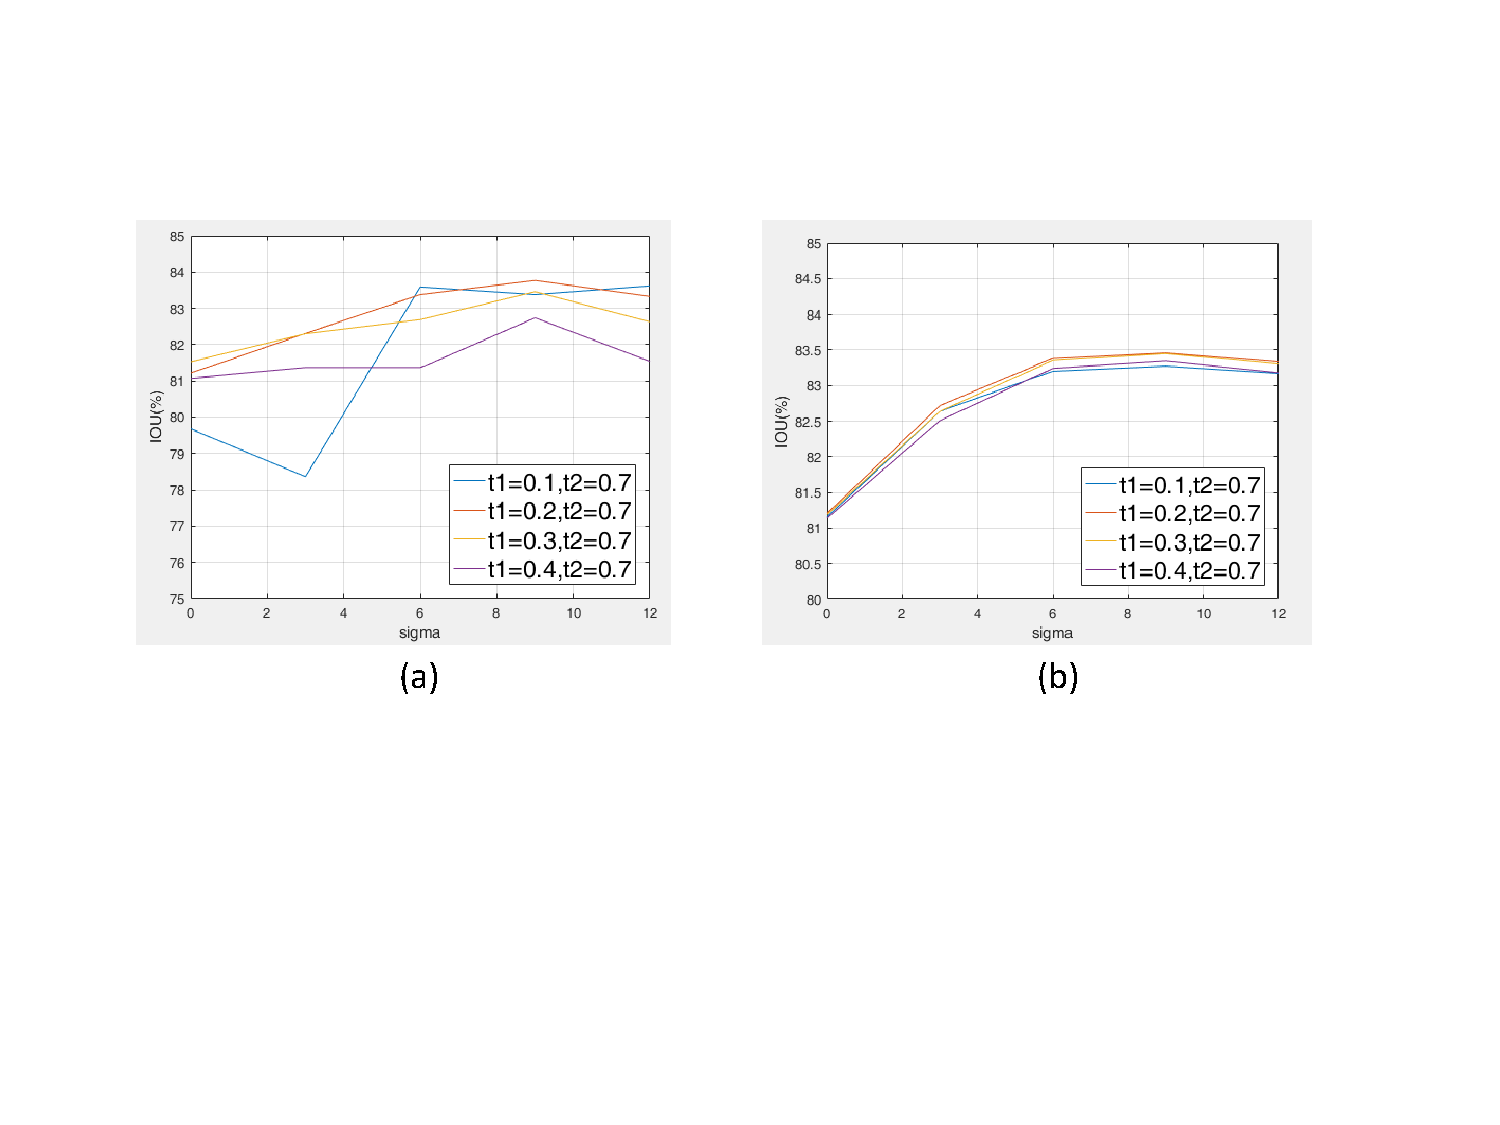
\includegraphics[width=3.3in]{figures/FigVar.pdf}
   %\includegraphics[width=0.8\linewidth]{egfigure.eps}
    \end{center}
    \caption{Effect of varying $\varepsilon$ for vesicle segmentation: (a)Fix $\tau_2$ and vary both $\tau_1$ and $\varepsilon$. (b) Fix $\tau_1$ and vary both $\tau_2$ and $\varepsilon$.}
    \label{FigVar}
\end{figure}


\noindent\textbf{Exploring the effect of $\{K, k_s, \tau_1, \tau_2\}$ to final segmentation.}
In this experiment, the effect of different $K$, $k_s$, $\tau_1$, $\tau_2$ for segmentation performance will be jointly investigated.
In order to reduce the hyper-parameters, we use $\varepsilon=\frac{(K-1)k_s}{2}$ to represent the effect of both $K$ and $k_s$ , because they have similar effects on SMP of changing the spreading range of a local maximum value.
Especially, $\varepsilon=0$ means no split max pooling applying to network.
Therefore, we first fix $\tau_2=0.7$ and vary $\tau_1$ to observe its influence of different $\varepsilon$ in DSAN model as shown in Figure~\ref{FigVar} (a).
Then, $\tau_1$ is fixed in turn and $\tau_2$, $\varepsilon$ are varied in Figure~\ref{FigVar} (b).
Observed from Figure~\ref{FigVar} , it is properly to employ $\varepsilon=9$ for vesicle segmentation to obtain most of the gains for different $\tau1$ and $\tau2$.
In practice, we set $k_s=9$ and $K=3$ to satisfy the condition of $\varepsilon=9$, because an overlarge $k_s$ or $K$ is harmful to efficiently implementing SMP.
For $\tau_1$ in Figure~ (a), we find that $\tau_1=0.2$ is the best lower threshold when $\varepsilon=9$.
And fixing $\tau_1=0.2$, $0.9$ is found to be optimal for $\tau_2$ according to Figure~\ref{FigVar} (b).
Finally, we use a large interval of $[0.2, 0.9]$ as the thresholds in Eq.~\ref{fusion} to impose a strong shape restriction on segmented synaptical vesicle objects.
Furthermore, the segmentation accuracy is found to be coarsely positive correlation to $\varepsilon$ in Figure~\ref{FigVar}, which demonstrates the effect of SMP on optimizing predicted shape parameters in boundary region.


\noindent\textbf{Qualitative evaluation on synaptic vesicle segmentation}
Figure \ref{FigVesicle} shows some segmentation results of testing data.
In order to verify the effectiveness of parameterized shape information, we compared our method with DeepLab~\cite{Chen2014a}, u-net~\cite{Ronneberger2015} without any complementary information and DCAN~\cite{Chen2016a} with contour map as auxiliary.
The fusing thresholds follow the optimal setting in previous experiment.

\begin{table}
\begin{center}
\begin{tabular}{lcc}
\hline
Method & F1($\%$) & IOU($\%$) \\
\hline
DeepLab & 66.75 & 80.95 \\
U-net & 69.99 & 77.56 \\
DCAN & 73.94 & 80.61 \\
DSAN- & 72.52 & 80.04 \\
DSAN & $\mathbf{75.68}$ & $\mathbf{83.34}$\\
\hline
\end{tabular}
\end{center}
\caption{The detection and segmentation results of different methods in our synaptic vesicle dataset.}
\label{tab:vesicle}
\end{table}


\begin{figure*}
    \begin{center}
        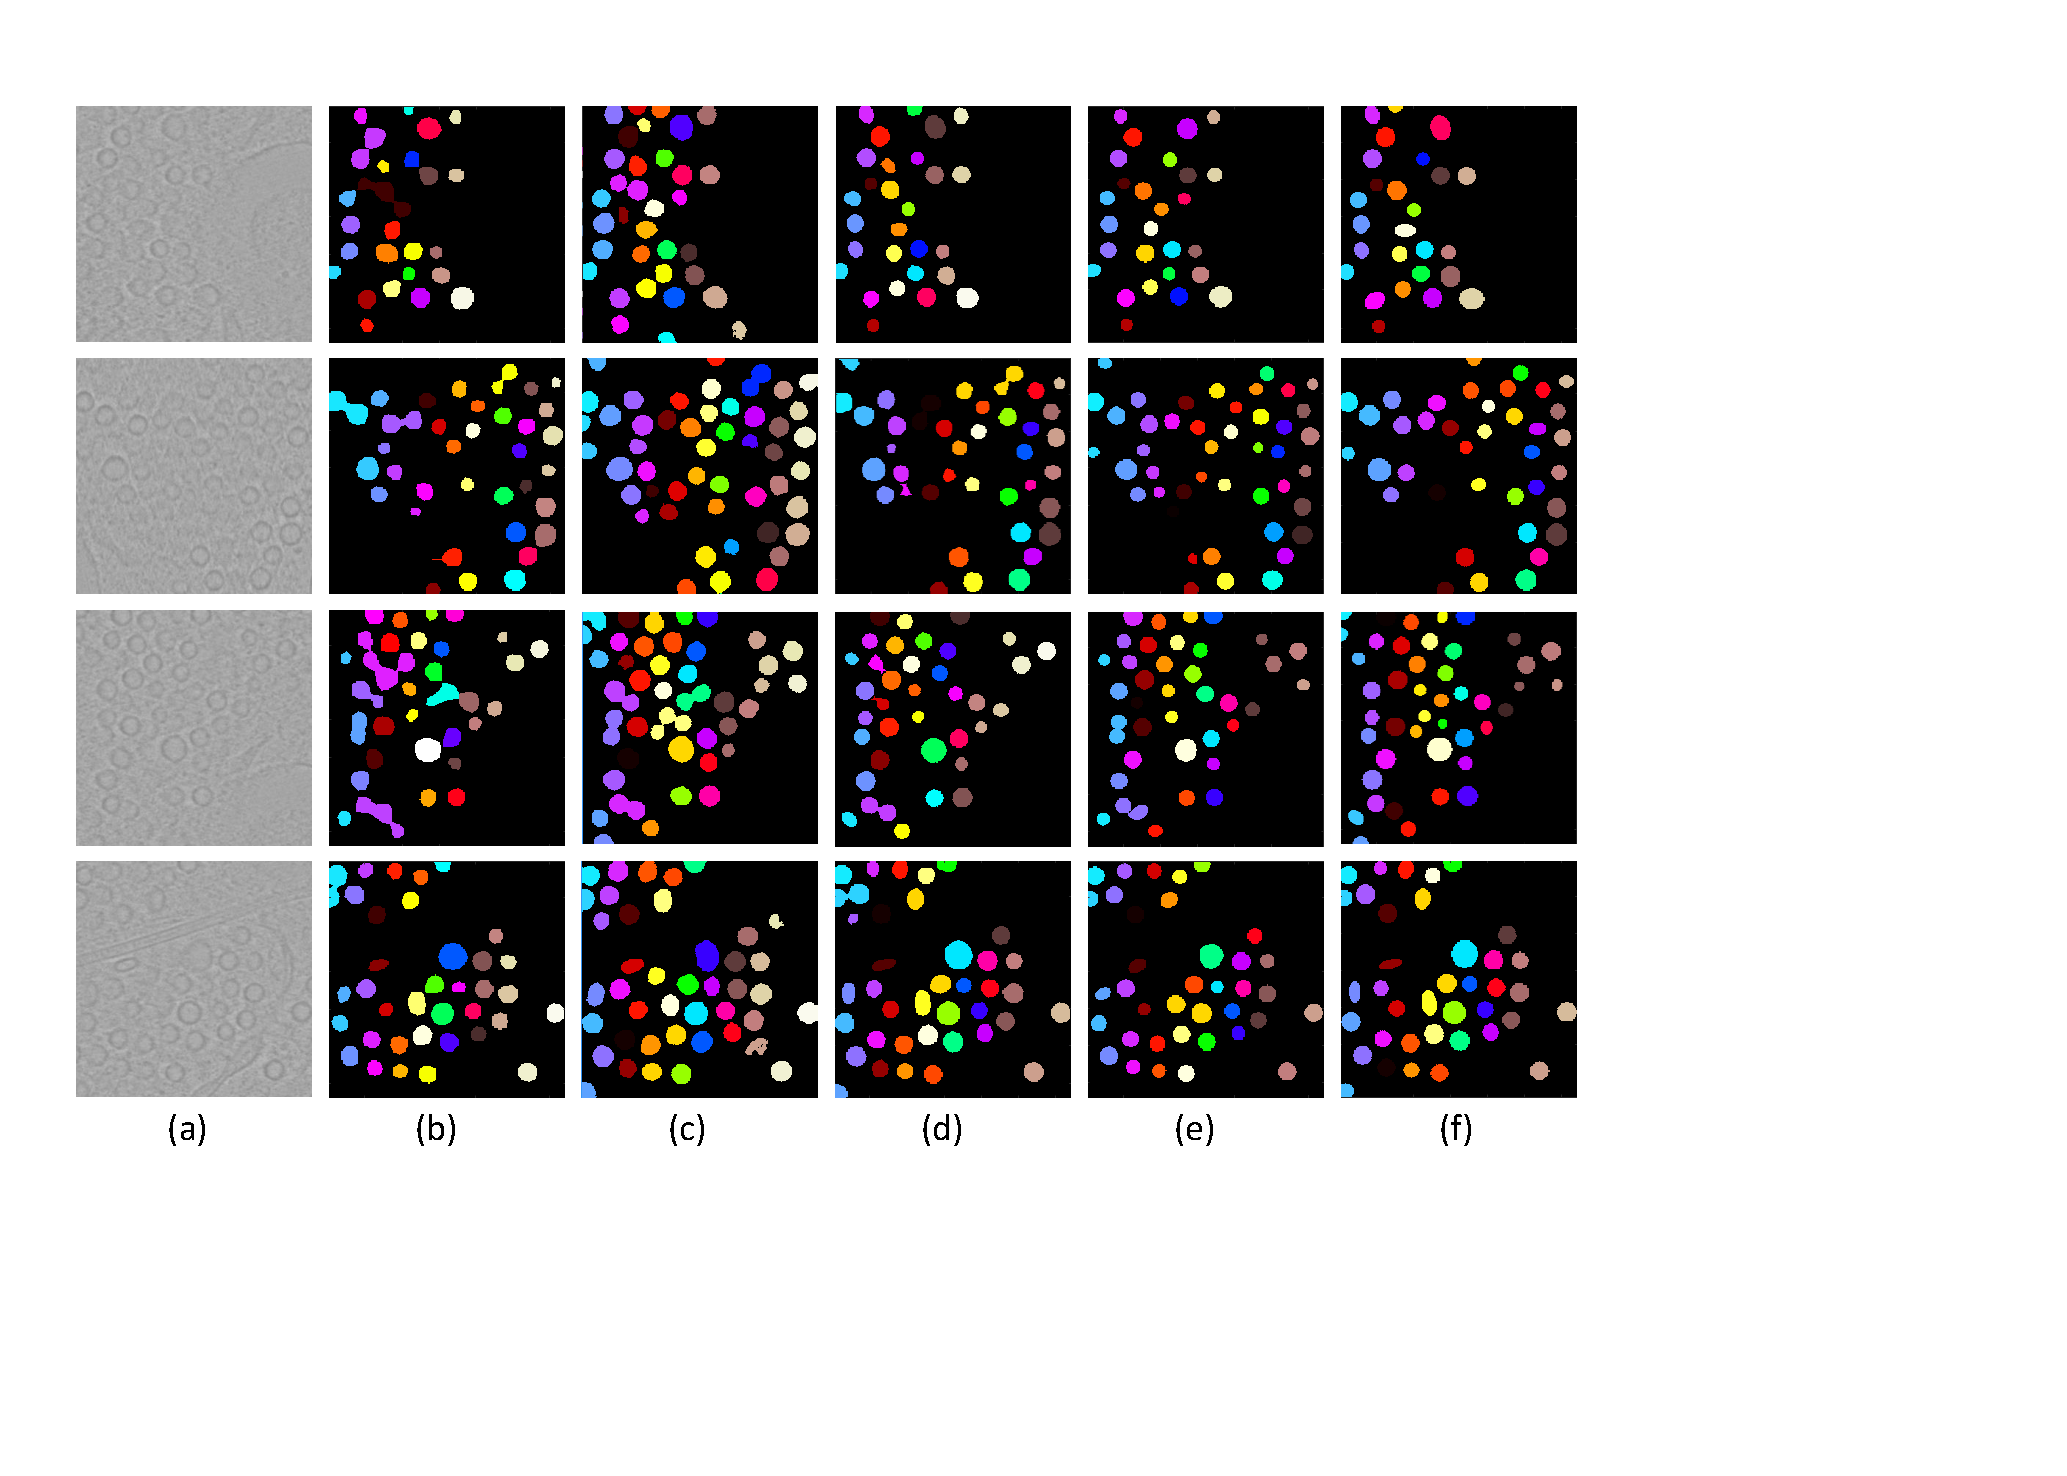
\includegraphics[width=6.8in]{figures/FigVesicle.pdf}
    \end{center}
    \caption{Some segmentation results of synaptic vesicle: (a) the input image; (b)-(e) the segmentation respectively from deeplab, u-net, DCAN and SCNN; (f) the ground truth.}
    \label{FigVesicle}
\end{figure*}

From Figure \ref{FigVesicle}, we can see that all the methods suffer from touching problem more or less in this experiment.
This is because that the contours of many synaptic vesicles are very fuzzy and incomplete due to deficient imaging technique, and the densely arrangement of objects also increases the challenging of clear segmentation as shown in Figure~\ref{FigVesicle} (a).
Both without auxiliary, u-net (Figure~\ref{FigVesicle} (c)) performs better than DeepLab due to the U-shape network that supplements many context information to higher resolutions layers, but the touching problem is still serious because of terrible image quality.
although DCAN can solve the touching problem in many tasks with the help of auxiliary contour prediction, the blurry boundary of objects in vesicle dataset make it much harder to obtain an accurate contour map, which results in the touching cases again in Figure~\ref{FigVesicle} (d).
Moreover, the predicted shape of objects by above methods are very coarse.
Differen from the above methods, our DSAN uses the shape parameters of objects as complementary information to separate the touching object clearly without residual regions.
As the results in Figure~\ref{FigVesicle} (e), almost all of the touching objects have been well separated apart and their shape are more smooth and regular.

However, an obvious drawback is that the large deviations of a certain shape parameter will cause a huge deformation of the final object shape in DSAN, as shown in last row of Figure~\ref{FigVesicle}.
Thus, a key emphasis of our subsequent work is to further improve the accuracy of predicted shape parameters.

\begin{figure}
    \begin{center}
        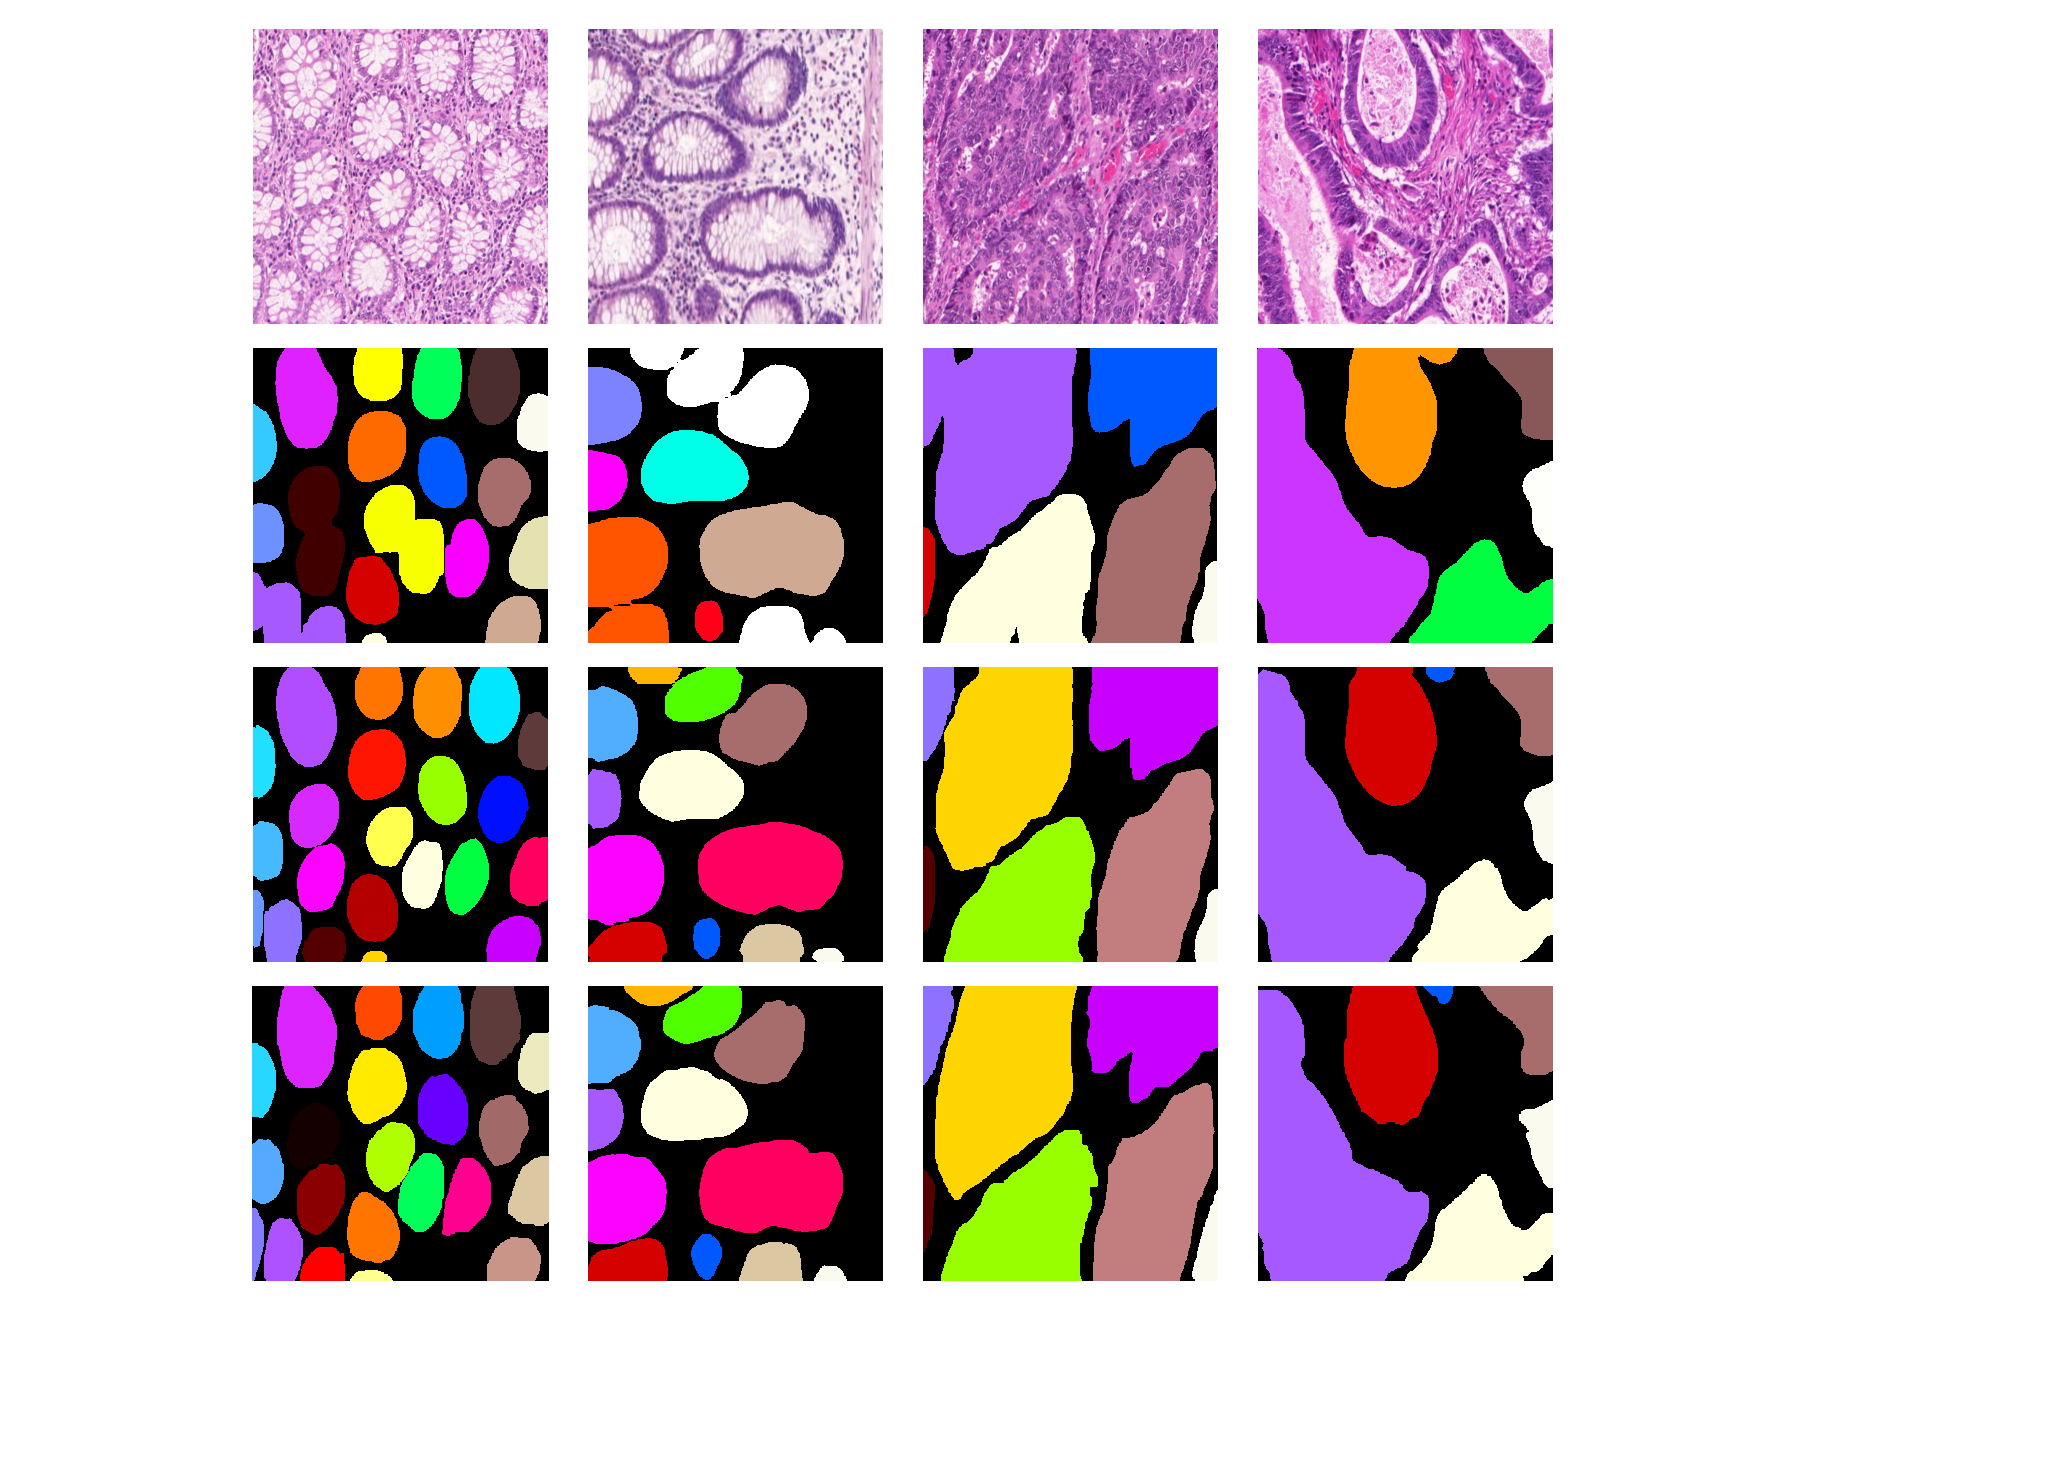
\includegraphics[width=3.4in]{figures/FigGland.pdf}
   %\includegraphics[width=0.8\linewidth]{egfigure.eps}
    \end{center}
    \caption{Several results of gland segmentation. 
    First two columns are the benign cases, and last two columns are the malignant cases.
    The results from top to bottom are original images, u-net, DSAN and ground truth.}
    \label{FigGland}
\end{figure}
\noindent\textbf{Quantitative evaluation.}
To quantitatively evaluate our method, we compare the object detection rate $F_1$ and the segmentation accuracy IOU of our SCNN with the state of the art segmentation methods based on Deeplab~\cite{Chen2014a}, u-net~\cite{Ronneberger2015} and DCAN~\cite{Chen2016b}, which are commonly used in biomedical image process.
Their results on our synaptic vesicle dataset are shown in Table~\ref{tab:vesicle}.
And we further implement DSAN- that is no SMP version of DSAN.
Their results are presented in Table~\ref{tab:vesicle} to prove superiority of our method.

From F1 score obtained in Table~\ref{tab:vesicle}, the performance of DSAN surpassed the other methods.
The common low F1 scores are caused by difficulty in detecting dense synaptical vesicles in such noise background.
Especially, we observed that the performance of u-net obtained about $3\%$ improvement over DeepLab, both of which did not use any auxiliary supervised information.
This arises from the fact that U-shape applied in u-net is effective to alleviate touching problem, which confirmed that missing of context information is a significant factor of touching problem in biomedical segmentation.
Furthermore, we noticed that there is not much improvement of F1 score obtained by DCAN compared to u-net and DeepLab.
This is because that many false detection region between two objects, separated by predicted contours, increase the false positive scores, shown in Figure~\ref{FigVesicle} (d).
And DSAN- gives a lower F1 score compared to DSAN, because of some touching cases caused by inaccurate auxiliary information predicted in boundary area.

From IOU metrics in Table~\ref{tab:vesicle}, our DSAN gives the best performance again among various methods.
It should be noted that although the other methods also obtain a good IOU score, their contours are more coarse and irregular as shown in Figure~\ref{FigVesicle}, which increase the difficulty of subsequent processing such as reconstruction of 3D structure.
And the segmented vesicle by our DSAN are more clear and regular.
Moreover, the results demonstrate that our split max pooling operation can effectively improve the accuracy of predicted shape parameters, which leads to a better performance on objects shape.
Both qualitative and quantitative evaluations present the superiority of our DSAN in segmenting densely arranged objects with regular and small objects by incorporating the prior shape knowledge into network.

\subsection{Gland segmentation}
\textbf{Dataset}
In this section we present DSAN for segmenting benign and malignant gland.
We consider the public dataset of \emph{Gland Segmentation Challenge Contest} in MICCAI2015~\cite{Sirinukunwattana2015a}.
The training dataset is composed of 85 images, consisting of 37 benign and 48 malignant, with ground truth annotations provided by expert pathologists.
The testing data contains two parts: 60 images for off-line evaluation and 20 images for on-site evaluation, and we put them together as our test dataset for evaluation.
Especially, there is a huge variation of glandular morphology in malignant case, which can prove the generalization of our DSAN to irregular objects.

\textbf{Implementation details}
Because of the many irregular objects in gland images, the prior shape constraint should be weaker on predicted objects shape by objectness.
Verified by experiment, we find that $\tau_2=0.7$ and $\tau_1=0.4 $ gives the best result of our DSAN in gland segmentation.
Especially, all the images are resized to $481\times 481$ as the input to our model following \cite{Chen2014a}.
The other experiments details are similar to the setting in vesicle segmentation.

\textbf{Qualitative evaluation on gland segmentation}
For qualitative evaluation, we present the results of u-net and DSAN in Figure~\ref{FigGland} to demonstrate the effect of shape parameters in separating touching objects apart and optimizing their shapes.
The first two columns are the examples of benign gland images, and the rest two columns are the examples of malignant images.
For benign gland cases in Figure~\ref{FigGland}, we can observed an obvious advantage of auxiliary shape information in separating dense regular objects.
And for some benign case, the predicted shape of irregular objects are also satisfied due to our piecewise fusion strategy, which retains the main shape predicted by objectness map.

\begin{table}
\begin{center}
\begin{tabular}{lcc}
\hline
		Method & F1 (\%) & Dice (\%) \\
		\hline
        CVIP Dundee &80.57& 83.11 \\
		u-net & 82.64 & 84.79 \\
		ExB1 & 85.16 & 85.82 \\
		DCAN & 86.26 & $\mathbf{86.83}$ \\
		DSAN & $\mathbf{86.58}$ & 86.10 \\
		\hline
\end{tabular}
\end{center}
\caption{The detection and segmentation results of different methods on gland segmentation dataset.}
\label{tab:gland}
\end{table}

\textbf{Quantitative evaluation}
Table \ref{tab:gland} shows the F1 score and object-level Dice index metric over \emph{Gland Segmentation Challenge Contest} by several published gland segmentation methods.
From the results, it can be seen that, with auxiliary shape parameters, the detection performance of our DSAN is the best, while the segmentation performance is slightly lower than DCAN.
The lower Dice score of DSAN than DCAN is caused by irregular glands in malignant cases, of which the predicted shapes are constrained by prior shape knowledge.
However, the holistic performance of DSCN is still conspicuous due to its superiority in separating touching objects apart and optimize the boundary of regular objects, while still accommodate seriously deformable objects.